\documentclass[12pt,a4paper]{amsart}
\usepackage{amsmath}
\usepackage{amssymb}
\usepackage{tikz}
\usetikzlibrary{decorations.markings}
\usetikzlibrary{shapes}
\usetikzlibrary{decorations.pathmorphing}
\usetikzlibrary{positioning}
\usetikzlibrary{cd}
\usetikzlibrary{calc}
\usetikzlibrary{backgrounds}
\usepackage{xcolor}
\tikzset{%
    symbol/.style={%
        draw=none,
        every to/.append style={%
            edge node={node [sloped, allow upside down, auto=false]{$#1$}}}
    }
}
\tikzset{->-/.style={decoration={
  markings,
  mark=at position .5 with {\arrow{>}}},postaction={decorate}}}
\tikzset{mid/.style 2 args={
        decoration={markings,
            mark= at position #2 with {\arrow{{#1}[scale=1.5]}} ,
        },
        postaction={decorate}
    },
mid/.default={>}{0.5}
}

\begin{document}

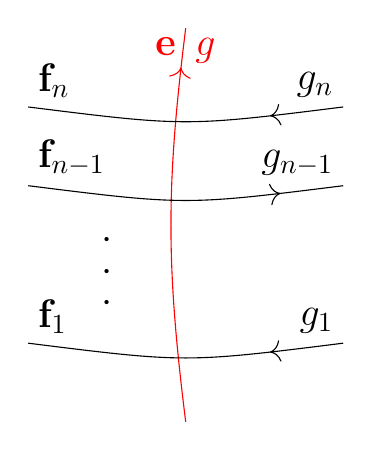
\begin{tikzpicture}
        \draw[mid={>}{0.9}, red] (3,0) .. controls ++(-0.25,2) and ++(-0.25,-2) .. (3,5) node[anchor=west, below right] {\Large $g$} node[anchor=east, below left] {\Large $\mathbf{e}$};
        \draw[mid={<}{0.8}] (1,1) node[anchor=south, above right] {\Large $\mathbf{f}_1$} .. controls ++(2,-0.25) and ++(-2,-0.25) .. (5,1)  node[anchor=south, above left] {\Large $g_1$};
        \draw[mid={>}{0.8}] (1,3) node[anchor=south, above right] {\Large $\mathbf{f}_{n-1}$} .. controls ++(2,-0.25) and ++(-2,-0.25) .. (5,3) node[anchor=south, above left] {\Large $g_{n-1}$};
        \draw[mid={<}{0.8}] (1,4) node[anchor=south, above right] {\Large $\mathbf{f}_n$} .. controls ++(2,-0.25) and ++(-2,-0.25) .. (5,4) node[anchor=south, above left] {\Large $g_n$};
        \node at (2,1.9) {\Large $\cdot$};
        \node at (2,1.5) {\Large $\cdot$};
        \node at (2,2.3) {\Large $\cdot$};
    \end{tikzpicture}

\end{document}